\section{Preliminary Work}
We have started implementing a form of active typechecking and translation, as outlined above, by developing an actively-typed programming language embedded within Python called Ace. In addition, we have demonstrated and empirically evaluated active code completion support for Java, implemented using class annotations and a  plugin for the Eclipse editor called Graphite.

\subsection{Ace: Active Typechecking and Translation}
Ace is an actively-typed programming language with a fixed syntax, shared with the Python language, but user-extensible semantics specified using an implementation of the active typing mechanism described above. The type-level language of Ace is Python, and types are type-level instances of Python classes implementing a provided interface, \verb|ace.Type|. The compiler selectively invokes the methods of these instances when type checking and translating expressions, a mechanism we call {\em active type-checking and translation (AT\&T)}. We have demonstrated the basic practicality of this mechanism by implementing primitives from several widely-known low-level languages, including much of C99 and the entirety of OpenCL, as active libraries. 
\begin{codelisting}
\lstinputlisting{listing4.py}
\caption{The generic \texttt{map} function compiled to map the \texttt{add5} function over two  types of input.}
\label{mapadd5dbl}
\end{codelisting}

\begin{codelisting}
\lstinputlisting{listing9.py}
\caption{A portion of the implementation of OpenCL pointer types implementing subscripting logic using the Ace extension mechanism.}
\label{pointers}
\end{codelisting}

An example showing usage of Ace with the OpenCL active library is shown in Listing \ref{mapadd5dbl}. Here, the top-level of the file is type-level code. On line 13, two instances of an active type, corresponding to the OpenCL types \verb|__global double*| and \verb|__global int*|, are created (to emphasize, at compile-time). The \emph{generic functions} defined on lines 4-11 are then programmatically specialized with these types assigned to the input arguments on lines 12-13, triggering active typechecking and translation mechanism when operations on these arguments are encountered (e.g. line 7).

Listing \ref{pointers} shows the portion of the implementation of the \verb|GlobalPtrType| type family (which \verb|A| and \verb|B| in Listing 1 are members of) that is responsible for the subscripting operation on line 7. The \verb|resolve_Subscript| method is responsible for checking that the subscript is an integer type, returning the appropriate type for the expression as a whole -- the target type of the pointer -- if so or raising an appropriate error if not. The \verb|translate_Subscript| function is then responsible for translating the subscript expression into the target language. Here, our target language is OpenCL (that is, we have simply lifted a target language construct into Ace directly), so the translation is straightforward. In general, however, this method may contain sophisticated code generation logic. These two methods correspond to the $f_{\text{resolve-X}}$ and $f_{\text{compile-X}}$ functions described above.
 
In addition to AT\&T, Ace supports more general forms of metaprogramming, and functions can be launched directly from Python with standard numeric data structures as arguments. Using Ace, we designed a scientific simulation framework that allows users to modularly specify, compile and orchestrate the execution of parameterized families of scientific simulations on clusters of GPUs. This framework has been used to successfully conduct large-scale, high-performance neuroscience simulations, providing initial evidence that Ace is useful not only as a foundational tool for researchers, but also for the practice of high-performance computing today.

\subsection{Graphite: Active Code Completion}\label{graphite}
Graphite demonstrates an edit-time aspect of active types, corresponding to the $f_{\text{editor}}$ function above, in the context of an existing language, Java, and an existing editor, Eclipse. A paper describing and evaluating this work which was recently published at ICSE 2012 \cite{omar2012active}. 
In that paper, we introduced {\em active code completion}, a mechanism that allows library developers to associate interactive and highly-specialized code generation interfaces, called {\em palettes}, directly with types using Java's annotation system and HTML5 for implementation. A simple example of such a palette and its operation is shown in Figure \ref{color}. 

Using several empirical methods, we examined the contexts in which such a system could be useful, described the design constraints governing the system architecture as well as particular code completion interfaces, and detailed the design of our implementation, Graphite. Using Graphite, we implemented a more sophisticated palette for writing regular expressions and conducted a small pilot study that showed that this kind of domain-specific interface is useful for professional developers working in that domain.

\begin{figure*}\label{color}
\begin{center}
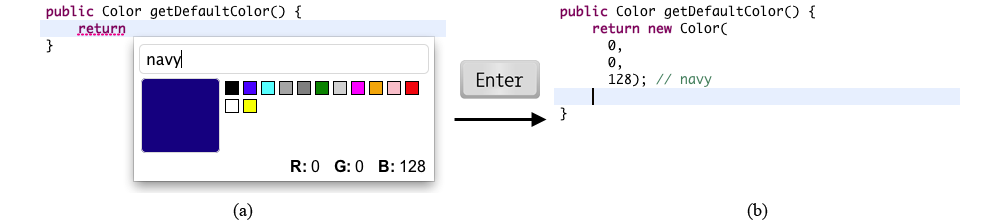
\includegraphics[width=40pc]{color_palette.png}\end{center}
\caption{(a) An example code completion palette associated with the \texttt{Color} class. (b) The source code generated by this palette.}
\end{figure*}
